\chapter{Ejercicios}
\section{Parcial I}
\begin{ejer}
    Resolver $y_{n+3} - 2y_{n+2} + 5/4 y_{n+1} - 1/2 y_n = 0$ con $y_0=1/2$, $y_1=1$, $y_2=0$.
\end{ejer} 
\begin{sol}
    $\underline{n=0} \Rightarrow y_3 = 2(0) - 5/4 + 1/4 = -1$.
$$p_c(x) = x^3 - 2x^2 + 5/4x - 1/2 = (x - 1/2)^2 (x - 1)$$
por lo que la soluci\'on en diferencias es $y_n = c_1(1/2)^n + c_2 n (1/2)^n + c_3 1^n$. Con las condiciones iniciales $y_i$ se pueden hallar los $c_i$. Adem\'as, la soluci\'on diferencial es
$$y(x) = c_1 e^{\frac{1}{2}x} + c_2 x e^{\frac{1}{2}x} + c_3 e^x$$
\end{sol}

\begin{ejer}
    Resolver $y'' + y = 0$.
\end{ejer} 
\begin{sol}
    Se tiene que el polinomio caracter\'istico es $p_c = x^2+1 = (x-i)(x+i)$ por tanto $\lambda_{1,2} = \pm i$, $\varrho = 1$, $\arctan 1/0 = \frac{\pi}{2}$. Las soluciones por tanto son
$$ y(x) = e^{x}\left(c_1 \cos \left( \frac{\pi}{2}x\right) + c_2 \sin \left( \frac{\pi}{2}x\right)\right) \qquad \qquad  y_n = c_1 \cos \left( \frac{\pi}{2}n\right)+ c_2 \sin \left( \frac{\pi}{2}n\right)$$
\end{sol}

\begin{ejer}
    $y'' = 0$.
\end{ejer}
\begin{sol}
    $y(x) = c_1 x + c_2$.
\end{sol}

\begin{ejer}
    Resolver $y^{(V)} - 4y^{(IV)} + 9y''' - 18y'' + 20y' + 8y = 0$.
\end{ejer}
\begin{sol}
    Se tiene que el polinomio caracter\'istico es $p_c(x) = x^5 - 4x^4 + 9x^3 - 18x^2 + 20x + 8 = (x-2i)(x+2i)(x-1)^2(x-2)$.
Llamando $\lambda_1 = 2i, \lambda_1^* = -2i$, $\varrho_1 = \sqrt{4+0} = 2$, $\theta_1 = \arctan(\pm \infty) = \pm \frac{\pi}{2}$. Por lo que las soluciones son
$$y(x) = e^{2x}\left[c_1 \cos \frac{\pi}{2} x + c_2 \sin \frac{\pi}{2} x + c_3 \cos(-\frac{\pi}{2} x) + c_4 \sin(-\frac{\pi}{2} x)\right] + e^x[c_5 + c_6 x] + c_7 e^{2x}$$
$$y_n = (2)^n \left[c_1 \cos \frac{\pi}{2}n + c_2 \sin \frac{\pi}{2}n + c_3 \cos(-\frac{\pi}{2}n) + c_4 \sin(-\frac{\pi}{2}n)\right] + c_5 1^n + c_6 n 1^n + c_7 2^n$$
\end{sol}


\begin{ejer}
    Pasar a sistema aut\'onomo la ecuaci\'on no lineal $y''+y=\sin(x)$.
\end{ejer}
\begin{sol}
    $$\begin{cases}
        y'=z\\ z'=y''=-y+\sin(x) \\ x'=1
    \end{cases} \iff \begin{pmatrix}
        y \\ z \\ x 
    \end{pmatrix}' = \begin{pmatrix}
        0 & 1 & 0 \\ -1 & 0 & 0 \\ 0 & 0 & 0
    \end{pmatrix} \begin{pmatrix}
        y \\ z \\ x 
    \end{pmatrix} + \begin{pmatrix}
        0 \\ \sin (x) \\ 1
    \end{pmatrix}$$ y ya es de la forma $Y' = F(Y)$.
\end{sol} 
\begin{ejer}
    Convertir en sistema aut\'onomo $y^{IV)} + y'' = \sin(y+x)$.
\end{ejer}
\begin{sol}
    $$\begin{cases}
        y'=y_1 \\ y_1'=y_2 \\ y_2' = y_3 \\ y_3'=y^{IV)}=-y_2 + \sin(y+x) \\ x'=1
    \end{cases}$$
\end{sol}
\begin{ejer}
    $y''+y=0$
\end{ejer}
\begin{sol} 
    Con su mapa de fases (gr\'afico de $y$ respecto de $y'$) es \begin{center}
    $\displaystyle
    \begin{cases}
        y'=z \\ z' = -y
    \end{cases} \iff \begin{pmatrix}
        y \\ z 
    \end{pmatrix}' = \begin{pmatrix}
        0 & 1 \\ -1 & 0
    \end{pmatrix} \begin{pmatrix}
        y\\ z
    \end{pmatrix}$%
    \qquad \qquad 
    \begin{tikzpicture}[baseline={(0,0)}, scale=0.42,
        trayectoria/.style={
            thick,
            blue,
            postaction={decorate},
            decoration={
                markings,
                mark=at position 0.125 with {\arrow{<}},
                mark=at position 0.375 with {\arrow{<}},
                mark=at position 0.625 with {\arrow{<}},
                mark=at position 0.875 with {\arrow{<}}
            }
        }
    ]
        % Cuadrícula de fondo
        \draw[lightgray, very thin, dashed] (-3.5,-3.5) grid (3.5,3.5);
        % Ejes principales
        \draw[->, thick] (-4, 0) -- (4, 0) node[right] {$y$};
        \draw[->, thick] (0, -4) -- (0, 4) node[above] {$y'$};
        % Trayectorias concéntricas
        \foreach \r in {1, 2, 3} {
            \draw[trayectoria] (0,0) circle (\r);
        }
        % Etiqueta del origen
        \node[below left] at (0,0) {$0$};
    \end{tikzpicture}
\end{center}
    
\end{sol}
\begin{ejer}
    Pasar a sistema $x^{IV)} + \omega^2 x t = \sin(t^2)$
\end{ejer}
\begin{sol}
    $$\begin{cases}
        x' = y_1 \\ y_1' = y_2 \\ y_2' = y_3 \\ y_3' = \sin(t^2) - \omega^2xt \\ y_4' = 1 \\ t'=1 
    \end{cases}$$
\end{sol}
\begin{obs}
    El sistema 
    $$\begin{cases}
        ^1y_{n+1} = \frac{2}{10} ^1y_n + ^2y_n \\ ^2y_{n+1} = ^1y_n +\frac{2}{10} ^2y_n
    \end{cases}$$
    es estable (no asint\'oticamente). En cambio en diferenciales es inestable.
\end{obs}
\begin{ejer}[1.5]
    Resolver $y'' - 2e^a \cos (\omega) y' + e^{2a} y=0$
\end{ejer}
\begin{ejer}
    [3.b] Pasar a sistema $x^{IV)} + \omega^2xt = \sin(t^2)$
\end{ejer}
\begin{sol}
    $$\begin{cases}
        x=z_o \\ x' = z_1=z_o' \\ z_1'=z_2 \\ z_2' = z_3 \\ z_3' = -\omega x z_4 + \sin(z_4^2) \\ z_4' = 1
    \end{cases}$$
\end{sol}
\begin{ejer}
    Comprobar la condici\'on de Lipschitz del ejemplo 3. y 5. 
\end{ejer}
\begin{sol}[3]
    $$y_{n+3} + \frac{1}{4}y_{n+2} - \frac{1}{2}y_{n+1} - \frac{3}{4}y_n = \frac{h}{8} \left[ 19 f(x_{n+2}, y_{n+2}) + 5 f(x_n, y_n) \right]$$$$
\phi_f = \frac{1}{8} \left[ 19 f(x_{n+2}, y_{n+2}) + 5 f(x_n, y_n) \right]
$$

\begin{enumerate}
    \item Comprobación para $f \equiv 0$. Si $f \equiv 0$, es evidente que $\phi_{f \equiv 0} = 0$
    \item Aplicación de la condición de Lipschitz. Evaluamos la diferencia de la función de incremento para dos soluciones $y$ e $y^*$:
    $$
    \|\phi_f(y, x; h) - \phi_f(y^*, x; h)\| = \left\| \frac{19}{8} f(x_{n+2}, y_{n+2}) + \frac{5}{8} f(x_n, y_n) - \left( \frac{19}{8} f(x_{n+2}, y^*_{n+2}) + \frac{5}{8} f(x_n, y^*_n) \right) \right\|
    $$
    Agrupando términos y aplicando la desigualdad triangular:
    $$
    \le \frac{19}{8} \|f(x_{n+2}, y_{n+2}) - f(x_{n+2}, y^*_{n+2})\| + \frac{5}{8} \|f(x_n, y_n) - f(x_n, y^*_n)\|
    $$
    Suponiendo que $f$ satisface la condición de Lipschitz con constante $L$:
    $$
    \le \frac{19}{8} L \|y_{n+2} - y^*_{n+2}\| + \frac{5}{8} L \|y_n - y^*_n\|
    $$
    Dado que $19/8 \le 3$ y $5/8 \le 3$, podemos acotarlo de forma global por $3L$:
    $$
    \le 3L \left( \|y_{n+2} - y^*_{n+2}\| + \|y_n - y^*_n\| \right)
    $$
    Por lo tanto, se cumple la condición requerida con la forma general $\sum M_j \|y_{n+j} - y^*_{n+j}\|$.
\end{enumerate}
\end{sol}
\begin{sol}[5]
Dada la función de incremento de un método de Runge-Kutta de 3 etapas:
$$ y_{n+1} - y_n= \frac{h}{4} (k_1 + 3k_3) \qquad  
\phi_f = \frac{1}{4} (k_1 + 3k_3)
$$
donde
$$
\begin{aligned}
    k_1 &= f(x_n, y_n) \\ 
    k_2 &= f\left(x_n + \frac{1}{3}h, \, y_n + \frac{1}{3}h k_1\right) \\ 
    k_3 &= f\left(x_n + \frac{2}{3}h, \, y_n + \frac{2}{3}h k_2 \right)
\end{aligned}
$$
\begin{enumerate}
    \item Comprobación para $f \equiv 0$:
    Si $f \equiv 0$, los términos $k_1$ y $k_3$ se anulan:
    $$
    \phi_{f \equiv 0} = \frac{1}{4} \left[ 0 + 3(0) \right] = 0
    $$

    \item Aplicación de la condición de Lipschitz:
    Queremos acotar la diferencia entre la función de incremento y su versión perturbada:
$$
\|\phi_f - \phi_f^*\| = \left\| \frac{1}{4} k_1 + \frac{3}{4} k_3 - \left( \frac{1}{4} k_1^* + \frac{3}{4} k_3^* \right) \right\| \le \frac{1}{4} \|k_1 - k_1^*\| + \frac{3}{4} \|k_3 - k_3^*\|
$$
\begin{enumerate}
    \item Acotación del primer término ($k_1$).
    
Dado que $k_1 = f(x_n, y_n)$ y $f$ cumple la condición de Lipschitz con constante $L$:
$$
\|k_1 - k_1^*\| = \|f(x_n, y_n) - f(x_n, y_n^*)\| \le L \|y_n - y_n^*\|
$$
\item Acotación del tercer término ($k_3$).

El término $k_3$ está definido como:
$$
k_3 = f\left(x_n + \frac{3}{2}h, \, y_n + \frac{2}{3}h f\left(x_n + \frac{1}{3}h, \, y_n + \frac{1}{3}h f(x_n, y_n)\right)\right)
$$
Para simplificar la notación interior, llamemos al argumento interno de la función de $k_3$ como $z_n$ y $z_n^*$:
$$
z_n = y_n + \frac{2}{3}h f\left(x_n + \frac{1}{3}h, \, y_n + \frac{1}{3}h f(x_n, y_n)\right)
$$

Aplicando la condición de Lipschitz a $k_3$ respecto a su segundo argumento:
$$
\|k_3 - k_3^*\| \le L \|z_n - z_n^*\|
$$
\item Desarrollo del término interior ($z_n$).
Sustituimos la definición de $z_n$ y aplicamos la desigualdad triangular junto con la condición de Lipschitz paso a paso:
$$
\|z_n - z_n^*\| = \left\| y_n - y_n^* + \frac{2}{3}h \left[ f\left(x_n + \frac{1}{3}h, \, y_n + \frac{1}{3}h f(x_n, y_n)\right) - f\left(x_n + \frac{1}{3}h, \, y_n^* + \frac{1}{3}h f(x_n, y_n^*)\right) \right] \right\|
$$
Aplicando Lipschitz a esta nueva evaluación de $f$:
$$
\|z_n - z_n^*\| \le \|y_n - y_n^*\| + \frac{2}{3}h L \left( \|y_n - y_n^*\| + \frac{1}{3}h \|f(x_n, y_n) - f(x_n, y_n^*)\| \right)
$$
Sustituyendo la acotación de $\|f - f^*\| \le L \|y_n - y_n^*\|$ dentro del paréntesis:
$$
\|z_n - z_n^*\| \le \|y_n - y_n^*\| + \frac{2}{3}h L \left( \|y_n - y_n^*\| + \frac{1}{3}h L \|y_n - y_n^*\| \right)
$$
Agrupando términos en función de $\|y_n - y_n^*\|$:
$$
\|z_n - z_n^*\| \le \left( 1 + \frac{2}{3}h L + \frac{2}{9}h^2 L^2 \right) \|y_n - y_n^*\|
$$
\item Sustitución final en $\phi_f$.
 
Ahora devolvemos este resultado a la acotación de $\|k_3 - k_3^*\|$ multiplicando por $L$:
$$
\|k_3 - k_3^*\| \le L \left( 1 + \frac{2}{3}h L + \frac{2}{9}h^2 L^2 \right) \|y_n - y_n^*\| = \left( L + \frac{2}{3}h L^2 + \frac{2}{9}h^2 L^3 \right) \|y_n - y_n^*\|
$$

Finalmente, combinamos todo en la expresión $\|\phi_f - \phi_f^*\| \le \frac{1}{4}\|k_1 - k_1^*\| + \frac{3}{4}\|k_3 - k_3^*\|$:
$$
\|\phi_f - \phi_f^*\| \le \left[ \frac{1}{4} L + \frac{3}{4} \left( L + \frac{2}{3}h L^2 + \frac{2}{9}h^2 L^3 \right) \right] \|y_n - y_n^*\|
$$
lo que demuestra que la función es de Lipschitz respecto a los valores de la solución numérica, garantizando la estabilidad del método.
\end{enumerate}
\end{enumerate}
\end{sol}
\begin{ejer}
    Comprobar la estabilidad del m\'etodo de Euler impl\'icito $y_{n+1} = y_n + hf_{n+1}$.
\end{ejer}
\begin{sol} \textbf{Consistencia.}
        $$\rho(x) = x-1 \Rightarrow \rho(1) = 1-1=0 \quad \checkmark$$
        $$\frac{\phi_f(y_n,x_n;0)}{\rho'(1)} =\frac{f(x_n,y_n)}{1} = f(x_n, y(x_n)) \quad \checkmark$$
       \textbf{Estabilidad}. $x-1$ tiene una ra\'iz real y es 1, siendo estable.
\end{sol}




\begin{ejer}
    [2.5.1] Dada la familia de métodos multipaso dependiente de $\alpha$:
$$
y_{n+2} + (\alpha - 1)y_{n+1} - \alpha y_n = \frac{h}{4} \left[ (\alpha + 3)f(x_{n+2}, y_{n+2}) + (3\alpha + 1)f(x_n, y_n) \right]
$$
\end{ejer}

\begin{enumerate}
    \item \textbf{Comprobación de la función de incremento y Lipschitz.}
    La función de incremento asociada es:
    $$
    \phi_f = \frac{1}{4} \left[ (\alpha + 3)f_{n+2} + (3\alpha + 1)f_n \right]
    $$
    Si $f \equiv 0$, se comprueba inmediatamente que $\phi_f = 0$. Para la condición de Lipschitz, evaluamos la diferencia acotada:
    $$
    \|\phi_f(y_n, y_{n+2}) - \phi_f(y_n^*, y_{n+2}^*)\| \le \frac{L}{4} \left[ (\alpha + 3)\|y_{n+2} - y_{n+2}^*\| + (3\alpha + 1)\|y_n - y_n^*\| \right]
    $$

    \item \textbf{Cero-estabilidad.}
    El polinomio característico asociado es:
    $$
    \rho(\zeta) = \zeta^2 + (\alpha - 1)\zeta - \alpha = (\zeta + \alpha)(\zeta - 1)
    $$
    Las raíces son $\zeta_1 = 1$ y $\zeta_2 = -\alpha$. Para garantizar la cero-estabilidad, debemos exigir que $|\alpha| < 1$ o bien $\alpha = 1$.

    \item \textbf{Consistencia.}
    Se verifica que $\rho(1) = 0$ y que se satisface la condición límite de consistencia para la función de incremento.
\end{enumerate}
\begin{ejer}[2.5.3]
Dado el método multipaso
$$
\begin{aligned}
    y_{n+2} &= \hat{y}_{n+2} - 6\alpha(y_{n+1} - y_n) + \alpha h(f_{n+2} - 4f_{n+3/2} + 7f_{n+1} + 2f_n) \\
    \hat{y}_{n+2} &= 2y_{n+1} - y_n + \frac{h}{3}(4f_{n+3/2} - 3f_{n+1} - f_n)
\end{aligned}
$$
Analizar su cero-estabilidad y la constante de Lipschitz.
\end{ejer}

\begin{sol}
\begin{enumerate}
    \item \textbf{Cero-estabilidad y polinomio característico:}
    El polinomio característico asociado al método es:
    $$
    \rho(\zeta) = \zeta^2 + (6\alpha - 2)\zeta - (6\alpha - 1)
    $$
     cuyas raíces son $\zeta_1 = 1$ y $\zeta_2 = 1 - 6\alpha$. 
    Para que el método sea cero-estable, las raíces deben satisfacer la condición del círculo unidad ($|\zeta| \le 1$ y las de módulo 1 simples):
    $$
    -1 \le 1 - 6\alpha \le 1 \implies -2 \le -6\alpha \le 0 \implies 0 \le \alpha \le \frac{1}{3}
    $$
    Sin embargo, si $\alpha = 0$, tendríamos una raíz doble en $\zeta = 1$, lo cual infringe la condición de cero-estabilidad. Por lo tanto, el rango válido es:
    $$
    \alpha \in \left(0, \frac{1}{3}\right)
    $$

    \item \textbf{Constante de Lipschitz ($M$).}
    Agrupando los términos de incremento y aplicando la acotación de Lipschitz, la constante $M$ del método queda expresada como:
    $$
    M = \left( \left|\alpha + \frac{4}{3}\right| - 4\alpha + |7\alpha - 1| + \left|2\alpha - \frac{1}{3}\right| \right) L^2
    $$
\end{enumerate}
\end{sol}
\begin{ejer}
Resolver mediante un método de Runge-Kutta de 2 etapas el PIV:
$$
\begin{cases}
    y'' + \omega^2 y = \varepsilon y^3 \\
    y(0) = 1, \quad y'(0) = 0
\end{cases}
$$
Comprobar la convergencia (hipótesis del método), convertir a sistema de primer orden, sacar sus puntos fijos y dar su mapa de fases ($\omega =1, \varepsilon=2$).
\end{ejer}

\begin{sol}
\begin{enumerate}
    \item \textbf{Comprobación de la convergencia (RK2 de 2 etapas)}
    El método de Runge-Kutta de 2 etapas utiliza la función de incremento:
    $$
    \phi_f = \frac{k_1 + k_2}{2}
    $$
    donde $k_1 = f(x_n, y_n)$ y $k_2 = f(x_n + h, y_n + h k_1)$.
    \begin{itemize}
        \item Si $f \equiv 0 \implies k_1 = 0, \, k_2 = 0 \implies \phi_f = 0$.
        \item Evaluando la condición de Lipschitz para la diferencia de incrementos:
        $$
        \|\phi_f - \phi_f^*\| = \left\| \frac{k_1 + k_2}{2} - \frac{k_1^* + k_2^*}{2} \right\| \le \frac{1}{2} (L\|y_n - y_n^*\| + L\|y_n - y_n^* + h(k_1 - k_1^*)\|)
        $$
        Desarrollando y acotando con la constante del método:
        $$
        \le \frac{2L + hL^2}{2} \|y_n - y_n^*\|
        $$
        Queda demostrado que cumple las hipótesis de Lipschitz y por tanto el método es convergente y cero-estable ($\rho(\zeta) = \zeta - 1$, con raíz simple en $\zeta = 1$).
    \end{itemize}

    \item \textbf{Conversión a sistema de primer orden.}
    Definimos $y_1 = y$ e $y_2 = y'$:
    $$
    \begin{cases}
        y_1' = y_2 \\
        y_2' = -\omega^2 y_1 + \varepsilon y_1^3
    \end{cases}
    $$
    con condiciones iniciales $y_1(0) = 1$, $y_2(0) = 0$.

    \item \textbf{Cálculo de puntos fijos.}
    Igualando las derivadas a cero:
    $$
    \begin{cases}
        y_2 = 0 \\
        -\omega^2 y_1 + \varepsilon y_1^3 = 0 \iff y_1(\varepsilon y_1^2 - \omega^2) = 0
    \end{cases}
    $$
    Obtenemos los tres puntos fijos en el espacio de fases:
    $$
    (0, 0), \quad \left(\frac{\omega}{\sqrt{\varepsilon}}, 0\right), \quad \left(-\frac{\omega}{\sqrt{\varepsilon}}, 0\right)
    $$
    \item \textbf{Mapa de fases}. Con $\omega=2$ y $\varepsilon=1$,
\begin{center}
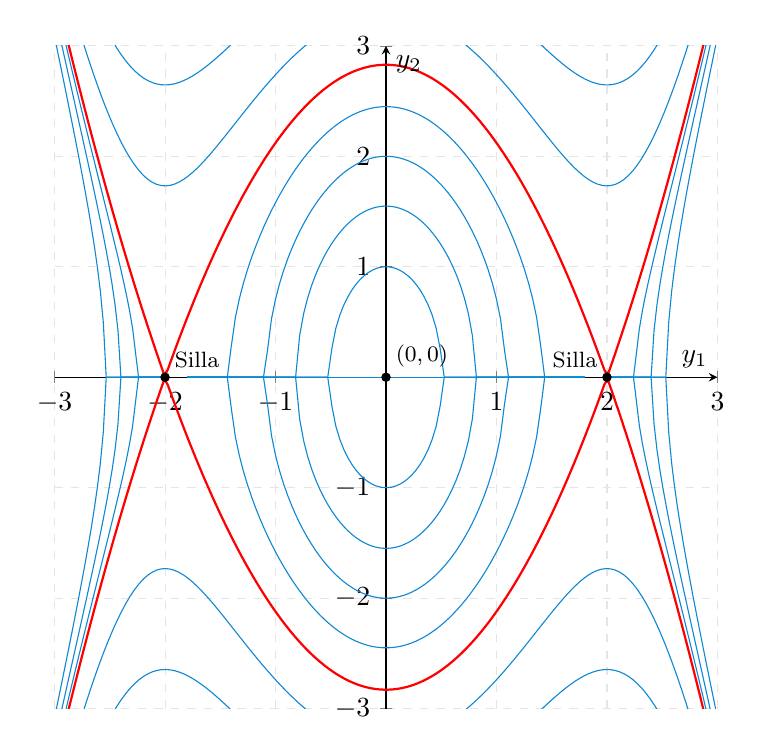
\begin{tikzpicture}
    \begin{axis}[
        xmin=-3, xmax=3,
        ymin=-3, ymax=3,
        axis lines=middle,
        xlabel={$y_1$},
        ylabel={$y_2$},
        samples=150,
        domain=-3.2:3.2,
        width=10cm,
        height=10cm,
        grid=both,
        grid style={dashed, gray!20}
    ]

        % 1. La Separatriz real (Energía C = 4, pasa por los puntos de silla +-2, 0)
        \addplot[domain=-3:3, samples=200, red, thick] ({x}, {sqrt(max(0, 2*(4 - 2*(x^2) + 0.25*(x^4))))});
        \addplot[domain=-3:3, samples=200, red, thick] ({x}, {-sqrt(max(0, 2*(4 - 2*(x^2) + 0.25*(x^4))))});

        % 2. Órbitas interiores cerradas (Centros alrededor del origen, C < 4)
        \foreach \C in {0, 0.5, 1.2, 2.0, 3.0} {
            \addplot[domain=-1.8:1.8, samples=100, cyan!70!blue, thin] ({x}, {sqrt(max(0, 2*(\C - 2*(x^2) + 0.25*(x^4))))});
            \addplot[domain=-1.8:1.8, samples=100, cyan!70!blue, thin] ({x}, {-sqrt(max(0, 2*(\C - 2*(x^2) + 0.25*(x^4))))});
        }

        % 3. Órbitas exteriores superiores e inferiores (C > 4)
        \foreach \C in {5.5, 7.5, 10.0, 14.0} {
            \addplot[domain=-3:3, samples=150, cyan!70!blue, thin] ({x}, {sqrt(max(0, 2*(\C - 2*(x^2) + 0.25*(x^4))))});
            \addplot[domain=-3:3, samples=150, cyan!70!blue, thin] ({x}, {-sqrt(max(0, 2*(\C - 2*(x^2) + 0.25*(x^4))))});
        }

        % 4. Órbitas adicionales en los laterales (trayectorias exteriores verticales para |y1| > 2)
        \foreach \C in {2.5, 3.2, 3.7} {
            \addplot[domain=2.001:4.1, samples=80, cyan!70!blue, thin] ({x}, {sqrt(max(0, 2*(\C - 2*(x^2) + 0.25*(x^4))))});
            \addplot[domain=2.001:4.1, samples=80, cyan!70!blue, thin] ({x}, {-sqrt(max(0, 2*(\C - 2*(x^2) + 0.25*(x^4))))});
            \addplot[domain=-4.1:-2.001, samples=80, cyan!70!blue, thin] ({x}, {sqrt(max(0, 2*(\C - 2*(x^2) + 0.25*(x^4))))});
            \addplot[domain=-4.1:-2.001, samples=80, cyan!70!blue, thin] ({x}, {-sqrt(max(0, 2*(\C - 2*(x^2) + 0.25*(x^4))))});
        }

        % 5. Puntos fijos (Centro en 0,0 y Sillas en +-2,0)
        \addplot[only marks, mark=*, mark size=1.5pt, black] coordinates {(0,0) (2,0) (-2,0)};
        
        % Etiquetas de los puntos fijos
        \node[above right, font=\footnotesize] at (axis cs:0,0) {$(0,0)$};
        \node[above left, font=\footnotesize] at (axis cs:2,0) {Silla};
        \node[above right, font=\footnotesize] at (axis cs:-2,0) {Silla};

        % Etiqueta de la separatriz
        \node[red, above, font=\small] at (axis cs:0, 3.2) {Separatriz};

    \end{axis}
\end{tikzpicture}
\end{center}
\end{enumerate}
\end{sol}


\section{Parcial II}


\begin{ejer}
    [5.5.1 (ii)] Consideremos $m = 2$, dado por $y = [u, v]^T$ y $f(y) = \left(\begin{smallmatrix} uv \\ u + v \end{smallmatrix} \right)$.
\end{ejer}
\begin{sol}
    \begin{itemize}
    \item \textbf{Orden 1:} $y^{(1)} = f(y) = \begin{pmatrix} uv \\ u + v \end{pmatrix}$
    \item \textbf{Orden 2:} Matriz Jacobiana $J(y)$ multiplicada por $f(y)$:
    \[
    y^{(2)} = \{f\} = f^{(1)}(f) = \begin{pmatrix} v & u \\ 1 & 1 \end{pmatrix} \begin{pmatrix} uv \\ u + v \end{pmatrix} = \begin{pmatrix} uv^2 + u^2 + uv \\ uv + u + v \end{pmatrix}
    \]
    \item \textbf{Orden 3:} Descomposición $y^{(3)} = \{f^2\} + \{\{f\}\}$:
    \begin{enumerate}
        \item \textit{Término $\{f^2\} = f^{(2)}(f, f)$:} Usando derivadas de 2º orden. Para $\!^1 f=uv$, las derivadas no nulas son cruzadas. Para $\!^2 f=u+v$ son nulas:
        \[
        f^{(2)}(f, f) = \begin{pmatrix} 0(uv)^2 + 2(1)(uv)(u+v) + 0(u+v)^2 \\ 0 \end{pmatrix} = \begin{pmatrix} 2uv(u+v) \\ 0 \end{pmatrix}
        \]
        \item \textit{Término $\{\{f\}\} = f^{(1)}(f^{(1)}(f))$:} Aplicando la Jacobiana al vector de orden 2:
        \[
        f^{(1)}(\{f\}) = \begin{pmatrix} v & u \\ 1 & 1 \end{pmatrix} \begin{pmatrix} uv^2 + u^2 + uv \\ uv + u + v \end{pmatrix} = \begin{pmatrix} v^3u + 2u^2v + uv^2 + u^2 + uv \\ uv^2 + u^2 + 2uv + u + v \end{pmatrix}
        \]
    \end{enumerate}
    Sumando ambos términos se obtiene la tercera derivada total exacta $y^{(3)}$ del sistema.
\end{itemize}
\end{sol}
\begin{ejer}
    [5.5.1 (iii)] Sistema Tridimensional (Cálculo tensorial). Consideremos $m = 3$, dado por $y = [u, v, w]^T$ y $f(y) = \left( \begin{smallmatrix} uvw \\ u(v+w) \\ v(v+w)  \end{smallmatrix}\right)$.
\end{ejer}
\begin{sol}
\begin{itemize}
    \item Derivadas de 1$^{er}$ orden (Jacobiana): ${\!^1}f_1 = vw, \, {\!^1}f_2 = uw, \, {\!^1}f_3 = uv \dots$
    \item Derivadas de 2º orden (${^i}f_{jk}$): Para $f^1$, solo las cruzadas no son nulas (${\!^1}f_{12}=w$, etc). Para $f^2$, ${^2}f_{12}={^2}f_{13}=1$. Para $f^3$, ${^3}f_{22}=2, {^3}f_{23}=1, {^3}f_{32}=1$.
    \item La primera diferencial elemental $\{f\}$ es:
    $$ \{f\} = \begin{pmatrix} 
        (vw)(uvw) + (uw)(u(v+w)) + (uv)(v(v+w)) \\ 
        (v+w)(uvw) + u(u(v+w)) + u(v(v+w)) \\ 
        0 + (2v+w)(u(v+w)) + v(v(v+w))
    \end{pmatrix} $$
\end{itemize}
\end{sol}


\begin{ejer}
Calcular la expresi\'on del siguiente \'arbol complejo
$$\begin{forest}
for tree={grow=north, circle, fill=black, inner sep=1pt, minimum size=2.5pt, l sep=10pt, s sep=8pt}
[ [ [ ] [ [] [ [] [] ] [] ] [ ] ] ]
\end{forest}$$
\end{ejer}
\begin{sol}
Las primeras 3 ramas son $[\tau^2]_2$, las siguientes $[[\tau^2]_2\tau^2]$ y por \'ultimo $[[[\tau^2]_2\tau^2] \tau^2]_2$.
\end{sol}


\begin{ejer}[5.7.2]
Demuestra que el m\'etodo siguiente tiene orden 4. Calcular $y'' + y = \frac{1}{10} y^3$ y ETL. 
\[
\begin{array}{c|ccc}
0           & 0             & 0             & 0             \\[0.5em]
\frac{1}{2} & \frac{5}{24}  & \frac{1}{3}   & -\frac{1}{24} \\[0.5em]
1           & \frac{1}{6}   & \frac{2}{3}   & \frac{1}{6}   \\
\hline
            & \frac{1}{6}   & \frac{2}{3}   & \frac{1}{6}
\end{array}
\]
\end{ejer}
\begin{sol}
\textbf{Orden 2:}
$$ \sum b_i = 1 \quad \checkmark $$
$$ [\tau] \rightsquigarrow \sum b_i c_i = \frac{1}{6}(0) + \frac{2}{3}\left(\frac{1}{2}\right) + \frac{1}{6}(1) = \frac{1}{2} \quad \checkmark $$

\textbf{Orden 3:}
$$ [\tau^2] \rightsquigarrow \sum b_i c_i^2 = \frac{1}{6}(0) + \frac{2}{3}\left(\frac{1}{4}\right) + \frac{1}{6}(1) = \frac{1}{3} \quad \checkmark $$
$$ [\tau]_2 \rightsquigarrow \sum b_i a_{ij} c_j = \frac{1}{6} \quad \checkmark $$

\textbf{Orden 4 (Ejemplo representativo):}
$$ [\tau^3] \rightsquigarrow \sum b_i c_i^3 = \frac{1}{6}(0) + \frac{2}{3}\left(\frac{1}{8}\right) + \frac{1}{6}(1) = \frac{1}{4} \quad \checkmark $$
$$ [\tau]_3 \rightsquigarrow \sum b_i a_{ij} a_{jk} c_k = \frac{1}{24} \quad \checkmark $$
Todas las condiciones de orden 4 se cumplen, comprobando que $\psi(t) = 1/\gamma(t)$. 

Para el orden 5 no se cumple. Por ejemplo para $[\tau^4]$ ($\gamma=5$):
$$ \psi([\tau^4]) = \sum b_i c_i^4 = \frac{2}{3}\cdot \frac{1}{16} + \frac{1}{6} \neq \frac{1}{5} $$
El método tiene orden estricto 4.
\end{sol}


\begin{ejer} 
Calcular un Runge-Kutta implícito de 2 etapas y la expresión del Error de Truncamiento Local (ETL) al integrar $y'' + y = y^2$. Programarlo.
\end{ejer}
\begin{sol} 
\noindent \textbf{Recordatorio.} El m\'etodo es impl\'icito si $a_{12}$ \'o $a_{22} \neq 0$. En general, si la \'ultima columna de $A$ tiene elementos no nulos. 

\textbf{1. Tablero de Butcher}
Para alcanzar orden 2 implícito con 2 etapas:
\[
\begin{array}{c|cc}
0   & 0   & 0   \\
1   & \frac{1}{2} & \frac{1}{2} \\
\hline
    & \frac{1}{2} & \frac{1}{2}
\end{array}
\]
Fórmula de avance temporal: $y_{n+1} = y_n + \frac{h}{2} [k_1 + k_2]$ donde $k_2 = f\left(x_n + h, y_n + \frac{h}{2}(k_1 + k_2)\right)$ (requiere un solucionador no lineal).

\textbf{2. Conversión a Sistema y Análisis del ETL}
Transformamos a $Y' = \begin{pmatrix} z \\ -y + y^2 \end{pmatrix}$.
Verificando condiciones de orden 3 ($\gamma([\tau^2])=3, \gamma([\tau]_2)=6$):
\[
\psi([\tau^2]) = \sum_{i} b_i c_i^2 = \frac{1}{2} \neq \frac{1}{3} \quad (\text{Falla, orden = 2})
\]
\[
\text{ETL} = \frac{h^3}{3!} \left[ \alpha([\tau^2]) (1-\gamma \psi) F([\tau^2]) + \alpha([\tau]_2) (1-\gamma \psi) F([\tau]_2) \right]
\]
Para el sistema dado, $\{f^2\} = \begin{pmatrix} 0 \\ 2z^2 \end{pmatrix}$ y $\{f\}_2 = \begin{pmatrix} (-1+2y)z \\ (-1+2y)(-y+y^2) \end{pmatrix}$.
Sustituyendo los valores de discrepancia:
$$\text{ETL} = -\frac{h^3}{12} \begin{pmatrix} (-1+2y)z \\ 2z^2(-1+2y)(-y+y^2) \end{pmatrix} + \mathcal{O}(h^4)$$
\end{sol}


\begin{ejer}[5.7.4] 
Escribe como m\'etodo RK, calcula el orden y la expresión del Error (ETL) al integrar $y'' + y = y^2$ del m\'etodo:
\begin{align*}
y_{n+\frac{2}{3}} &= y_n + \frac{h}{3} \left[ f(y_{n+\frac{2}{3}}) + f(y_n) \right] \\
y_{n+1} &= y_n + \frac{h}{4} \left[ 3f(y_{n+\frac{2}{3}}) + f(y_n) \right]
\end{align*}
\end{ejer}
\begin{sol}
\textbf{1. Tablero de Butcher:}
Extrayendo coeficientes de las ecuaciones de $k_1$ y $k_2$:
\[
\begin{array}{c|cc}
0           & 0          & 0          \\
\frac{2}{3} & \frac{1}{3}& \frac{1}{3} \\ \hline
            & \frac{1}{4}& \frac{3}{4}
\end{array}
\]
Condiciones:
\begin{itemize}
    \item \textbf{Orden 1:} $\sum b_i = 1 \checkmark$
    \item \textbf{Orden 2:} $\sum b_i c_i = \frac{1}{2} \checkmark$
    \item \textbf{Orden 3:} $\psi([\tau^2]) = \frac{1}{3} \checkmark, \quad \psi([[\tau]]) = \frac{1}{6} \checkmark$
    \item \textbf{Orden 4:} $\psi([\tau^3]) = \frac{2}{9} \neq \frac{1}{4} \cross$ (Falla).
\end{itemize}
El método tiene orden estricto 3.
\end{sol}



\begin{ejer}[5.8.3] 
Calcula el orden y el LTE. Si es escalar calcular tambi\'en el orden y decir por qu\'e es distinto.  
\begin{enumerate}[i)]
    \item Deducir de la siguiente tabla que cuando un método de Runge-Kutta de cuarto orden se aplica a una ecuación escalar $y' = f(y)$, cuatro de las diferenciales elementales que aparecen en la expresión para el error de truncamiento local principal (PLTE) se reducen a la misma expresión $\phi(t)$. \footnote{p.174 Lambert}
    \begin{center}
$\begin{array}{c|cccc}
0 & \\
\frac{1}{2} & \frac{1}{2} \\
-1 & \frac{1}{2} & -\frac{3}{2}   \\
1 & 0 & \frac{4}{3} & -\frac{1}{3} \\
\hline
& \frac{1}{6} & \frac{2}{3} & 0 & \frac{1}{6}
\end{array}$
\end{center}
    \item Considere el método explícito:
\begin{center}
$\begin{array}{c|cccc}
0 & \\
\alpha & \alpha & \\
\frac{1}{2} & \frac{1}{2} - \frac{1}{8\alpha} & \frac{1}{8\alpha} &  \\
1 & \frac{1}{2\alpha} - 1 & -\frac{1}{2\alpha} & 2 &  \\
\hline
& \frac{1}{6} & 0 & \frac{2}{3} & \frac{1}{6}
\end{array}$
\end{center}
Demuestre que para todos los valores de $\alpha$ el orden es \emph{precisamente} cuatro cuando se aplica al sistema general $y' = f(y)$, $f \in \mathbb{R}^m$. En el caso en que $m = 1$, encuentre el valor de $\alpha$ para el cual el coeficiente de $\phi(t)$, definido en (i), es cero.
\end{enumerate}
\end{ejer}

\begin{sol}
\subsubsection*{Parte (i): Verificación del orden y cálculo del ETL}
Evaluamos los sumatorios de Butcher (que denotaremos como $\psi$):

\begin{itemize}
    \item \textbf{Orden 1:} 
    \[
    \psi(\tau) = \sum_{i=1}^4 b_i = \frac{1}{6} + \frac{2}{3} + 0 + \frac{1}{6} = 1 \quad (\checkmark \text{ Se cumple})
    \]
    \item \textbf{Orden 2:} 
    \[
    \psi ([\tau]) = \sum_{i=1}^4 b_i c_i = \frac{1}{6}(0) + \frac{2}{3}\left(\frac{1}{2}\right) + 0(-1) + \frac{1}{6}(1) = \frac{1}{3} + \frac{1}{6} = \frac{1}{2} \quad (\checkmark \text{ Se cumple})
    \]
    \item \textbf{Orden 3:} 
    \begin{align*}
        \psi ([\tau^2])  &= \sum_{i=1}^4 b_i c_i^2 = \frac{2}{3}\left(\frac{1}{4}\right) + \frac{1}{6}(1) = \frac{1}{3} \quad (\checkmark) \\
        \psi ([\tau]_2)  &= \sum_{i=1}^4 b_i \sum_{j=1}^4 a_{ij} c_j = \frac{1}{6} \quad (\checkmark)
    \end{align*}
    \item \textbf{Orden 4 (Donde se produce el fallo):}
    \begin{align*}
        \psi ([\tau^3])  &= \sum_{i=1}^4 b_i c_i^3 = \frac{1}{4} \quad (\checkmark) \\
        \psi ([\tau[\tau]]) &= \sum_{i=1}^4 b_i c_i \sum_{j=1}^4 a_{ij} c_j = \frac{1}{6} \neq \frac{1}{8} \quad (\mathbf{\text{Falla}}) \\
        \psi ([\tau^2]_2) &= \sum_{i=1}^4 b_i \sum_{j=1}^4 a_{ij} c_j^2 = 0 \neq \frac{1}{12} \quad (\mathbf{\text{Falla}}) \\
        \psi ([\tau]_3) &= \sum_{i=1}^4 b_i \sum_{j=1}^4 \sum_{k=1}^4 a_{ij} a_{jk} c_k = \frac{1}{24} \quad (\checkmark)
    \end{align*}
\end{itemize}

Como las condiciones de orden 4 fallan, el método tiene un \textbf{orden estricto $p = 3$}.

\subsection*{Cálculo del Error de Truncamiento Local (ETL)}
Utilizando la formulación en función de los sumatorios $\psi(t)$, $\alpha(t)$ y las densidades de los árboles elementales $\gamma(t)$ multiplicadas por las derivadas de Fréchet
\begin{align*}
\text{ETL} & = \frac{h^4}{4!} \sum_{r(t)=4} \alpha(t) \left( 1-\psi(t) \gamma(t) \right) F(t) + \mathcal{O}(h^5) \\
&= \frac{h^4}{4!}  \left[ 3 \left( 1- \psi ([\tau[\tau]]) \cdot 8 \right) \{f\{f\}\} + 1 \left(  1 -\psi ([\tau^2]_2) \cdot 12 \right)\{\{f^2\}\} \right] \\
&= \frac{h^4}{4!}  \left[ 3 \left( 1- \frac{1}{6} \cdot 8 \right) \{f\{f\}\} + \left( 1- 0 \cdot 12 \right)\{\{f^2\}\} \right] \\
&= \frac{h^4}{4!}  \left[ 3 \left( \frac{6-8}{6}  \right) \{f\{f\}\} +  \{f^2\}_2 \right] \\
&= \frac{h^4}{4!}  \left[ 3 \left( \frac{-1}{3}  \right) \{f\{f\}\} +  \{f^2\}_2 \right] \\
&= \frac{h^4}{4!}  \left[ - \{f\{f\}\} + \{f^2\}_2 \right] + \mathcal{O}(h^5)
\end{align*}
y si $m=1$, es decir, trabajamos en $\bb R^1$, en ese caso $\{f\} = f_y f$, luego $\{f\}_2 = f_y f_{yy} f^2 = f_{yy} f f_{y} f = \{f\{f\}\}$ \hyperref[ap1]{Tabla 5.5}, y entonces ETL $= \mc O(h^5)$ y el m\'etodo es de orden 4. 

\subsubsection*{Parte (ii): Verificación del orden 4 y posible orden 5}
Para que el método alcance el orden 4 de forma general, debe satisfacer exactamente las ecuaciones de los árboles elementales de Butcher hasta orden 4. Con los vectores $c = [0, \alpha, \nicefrac{1}{2}, 1]^T$ y $b = [\nicefrac{1}{6}, 0, \nicefrac{2}{3}, \nicefrac{1}{6}]^T$, evaluamos analíticamente las condiciones:

\begin{itemize}
    \item \textbf{Orden 1:} $\sum b_i = \frac{1}{6} + 0 + \frac{2}{3} + \frac{1}{6} = 1$
    \item \textbf{Orden 2:} $\sum b_i c_i = \frac{2}{3}\left(\frac{1}{2}\right) + \frac{1}{6}(1) = \frac{1}{2}$
    \item \textbf{Orden 3:} 
    \begin{align*}
        \sum b_i c_i^2 &= \frac{2}{3}\left(\frac{1}{4}\right) + \frac{1}{6}(1) = \frac{1}{3} \\
        \sum b_i a_{ij} c_j &= \frac{2}{3}\left(\frac{1}{8\alpha} \alpha\right) + \frac{1}{6}\left(-\frac{1}{2\alpha} \alpha + 2 \cdot \frac{1}{2}\right) = \frac{1}{12} + \frac{1}{12} = \frac{1}{6}
    \end{align*}
    \item \textbf{Orden 4:}
    \begin{align*}
        \sum b_i c_i^3 &= \frac{2}{3}\left(\frac{1}{8}\right) + \frac{1}{6}(1) = \frac{1}{4} \\
        \sum b_i c_i a_{ij} c_j &= \frac{2}{3}\left(\frac{1}{2}\right)\left(\frac{1}{8}\right) + \frac{1}{6}(1)\left(\frac{1}{2}\right) = \frac{1}{8} \\
        \sum b_i a_{ij} c_j^2 &= \frac{2}{3}\left(\frac{1}{8\alpha} \alpha^2\right) + \frac{1}{6}\left(-\frac{1}{2\alpha} \alpha^2 + 2 \cdot \frac{1}{4}\right) = \frac{\alpha}{12} - \frac{\alpha}{12} + \frac{1}{12} = \frac{1}{12} \\
        \sum b_i a_{ij} a_{jk} c_k &= \frac{1}{6}\left(2 \cdot \frac{1}{8}\right) = \frac{1}{24}
    \end{align*}
    \item \textbf{Orden 5:}
    \begin{align*} 
        \sum_{i=1}^4 b_i \sum_{j=1}^4 a_{ij} \sum_{k=1}^4 a_{jk} c_k^2 &= b_4 \sum_{j=1}^4 a_{4j} \left( \sum_{k=1}^4 a_{jk} c_k^2 \right) = b_4 \left( a_{42} \sum_{k=1}^4 a_{2k} c_k^2 + a_{43} \sum_{k=1}^4 a_{3k} c_k^2 \right) \\ 
        &= \frac{1}{6} \left[ a_{42}(0) + a_{43} \left( a_{31} c_1^2 + a_{32} c_2^2 \right) \right] = \frac{1}{6} \left[ 2 \left( \left(\frac{1}{8\alpha}\right) \alpha^2 \right) \right] \\
        &= \frac{1}{6} \left[ 2 \left( \frac{\alpha}{8} \right) \right] = \frac{1}{6} \left( \frac{\alpha}{4} \right) = \frac{\alpha}{24} = \frac{1}{60} \iff \alpha=\frac{2}{5} 
    \end{align*}
\end{itemize}
Dado que todas las identidades hasta orden 4 se cumplen de manera exacta sin depender del parámetro $\alpha$ (siempre que $\alpha \neq 0$), queda demostrado que el método tiene precisamente orden 4 para cualquier sistema general multidimensional $f \in \mathbb{R}^m$. Para alcanzar orden 5 (en los sumatorios que dependen de $\alpha$), hay que imponer condiciones restrictivas como $\alpha = \frac{2}{5}$.
\end{sol}





